\documentclass[12pt,a4paper]{article}

\usepackage[utf8]{inputenc}
\usepackage[greek,english]{babel}
\usepackage{alphabeta} 

\usepackage[pdftex]{graphicx}
\usepackage[top=1in, bottom=1in, left=1in, right=1in]{geometry}
\linespread{1.06}
\setlength{\parskip}{8pt plus2pt minus2pt}

\widowpenalty 10000
\clubpenalty 10000

\newcommand{\eat}[1]{}
\newcommand{\HRule}{\rule{\linewidth}{0.5mm}}

\usepackage[official]{eurosym}
\usepackage{enumitem}
\setlist{nolistsep,noitemsep}
\usepackage[hidelinks]{hyperref}
\usepackage{cite}
%\usepackage{lipsum}


\begin{document}
	
	%===========================================================
	\begin{titlepage}
		\begin{center}
			
			% Top 
			
\includegraphics[width=0.55\textwidth]{the-university-of-sydney-vector-logo.png}~\\[2cm]
			
			
			% Title
			\HRule \\[0.4cm]
			{ \LARGE 
				\textbf{Project Report for ENGG2112}\\[0.4cm]
				\emph{Towards Robust Fake News Detection: A Comprehensive Machine Learning Study}\\[0.4cm]
			}
			\HRule \\[1.5cm]
			
			
			
			% Author
			{ \large
				Lam Duy Nhat Le, 510670000, Software Engineering \\[0.1cm]
				RueiEn Tan, 480421111, Software Engineering\\[0.1cm]
				Yijiang Luo, 49052222, Software Engineering\\[0.1cm]
				Shuaiyu Lu, SID, Software Engineering\\[0.1cm]
			}
			
			\vfill
			
			\textsc{\large Faculty of Engineering}\\[0.4cm]
			
			
			% Bottom
			{\large \today}
			
		\end{center}
	\end{titlepage}
	
	\begin{center}
%		\lipsum[1-2]

	\subsection*{Executive Summary}
	\end{center}
	
	\noindent Put your executive summary here. Its purpose is to summarize the objectives, methodology, main findings and conclusions of the project. Its intended audience is a reader who does not have enough time to read the main body of the report carefully, usually a busy executive, hence the name.
	
%	\addcontentsline{toc}{ }{Executive Summary}

	
	\newpage
	
	
	
	%===========================================================
	\tableofcontents
	\addtocontents{toc}{\protect\thispagestyle{empty}}
	\newpage
	\setcounter{page}{1}
	
	%===========================================================
	%===========================================================
	\section{Background and Motivation}\label{sec:intro}

	In today's digital age, the internet has become the cornerstone of information dissemination, reaching two-thirds of the global population [1]. While this connectivity has revolutionized the way we access and share information, it has also risen an abundance of challenges, most notably the spread of misinformation or ``fake news''. The adage ``don't trust everything on the internet'' has never been more relevant, yet the sophistication with which misinformation is created and disseminated has made it increasingly difficult for individuals to discern fact from fiction. Recent studies indicate that more than 40\% of news articles shared on social media platforms are misleading or entirely false, underscoring the gravity of this issue [2].

	The role of machine learning in this context is paradoxical. On one hand, machine learning technologies offer promising avenues for automated fact-checking and fake news detection. On the other hand, these identical machine learning technologies possess the capacity to generate highly credible disinformation in the form of counterfeit news articles, manipulated visual content, and fabricated video material that convincingly mimics the appearance and speech of public figures. This dual role creates a complex landscape where the tools for both generating and combating misinformation are continuously evolving.

As undergraduate students in Software Engineering, we find ourselves at the intersection of this technological and ethical landscape. Software engineering principles are deeply embedded in the algorithms that both generate and detect misinformation. Therefore, we believe it is not just an opportunity but a responsibility for us to contribute to this field. Our project aims to develop a robust machine learning model capable of discerning the authenticity of various types of articles, be it news stories, blogs, or opinion pieces. By incorporating multiple features such as the text, title, and authorship into our model, we aspire to improve the accuracy and reliability of fake news detection algorithms.

For this research, we have chosen a dataset provided by the UTK Machine Learning Club and made available on Kaggle as part of a competition. We opted for this dataset for several reasons:
\begin{itemize}
	\item \textsf{Size}: With 20,000 entries, the dataset is sufficiently large to train and test machine learning models effectively.
	\item \textsf{Cleanliness}: The dataset is well-curated, reducing the amount of preprocessing required, which is often a time-consuming step in machine learning projects.
	\item \textsf{Comprehensiveness}: It includes multiple features such as the text, title, and author, along with labels indicating whether the news is fake or not. This allows for a multi-faceted approach to the problem.
\end{itemize}

Through this research, we hope to make a meaningful contribution to the ongoing efforts to combat misinformation, thereby fostering a more informed and trustworthy digital ecosystem.
	\section{Objectives and Problem Statement}\label{sec:prob}
	The primary objective of our research is to develop a machine learning model capable of determining the trustworthiness of news articles. To achieve this, we aim to utilize a range of feature extraction techniques and machine learning models. Specifically, we plan to explore various approaches to feature extraction, including Term Frequency-Inverse Document Frequency (TF-IDF), N-Gram analysis, and Sentiment Analysis. For model training, we intend to employ four different machine learning algorithms: Naive Bayes Classifier, K-Nearest Neighbour, Support Vector Machines, and Neural Networks.

	The choice of multiple feature extraction techniques and machine learning models is motivated by the inherent complexities and nuances in fake news detection. Different approaches to feature extraction have their own advantages and limitations. For instance, TF-IDF has been effective in capturing the importance of terms in text documents, while N-Gram analysis has shown promise in capturing contextual information in textual data [3]. Sentiment Analysis, on the other hand, can provide insights into the emotional tone of the text, which could be a crucial factor in determining its credibility.

	Similarly, using multiple machine learning models allows us to leverage the strengths of each. Naive Bayes and K-Nearest Neighbour are good at sorting text into different categories, while Support Vector Machines excel at handling complex data with many variables [3]. Neural Networks offer the advantage of learning complex patterns in the data, which could be particularly useful in fake news detection.

	The problem we aim to solve is to identify the most effective combination of feature extraction techniques and machine learning models for fake news detection. The ultimate goal is to find the method and model that yield the highest accuracy in classifying news articles as trustworthy or not. This is crucial given the increasing prevalence of misinformation and the varying effectiveness of existing models in the literature [4].
%	\lipsum[3-4]\cite{einstein}
	
	\section{Methodology}\label{sec:meth}
	\subsection{Data Pre-Processing}
	As some of the independent variables are categorical in nature, we first need to use one-hot encoding to convert them to (binary) numerical variables. There are also a number of missing data values, which we replace with zero where appropriate\footnote{These are those variables which are blank because their true values are zero.} and with the average value of that variable calculated using the non-empty values otherwise. These were implemented using the \textsf{sklearn} module's functions, as follows:
	\begin{enumerate}
		\item \textsf{onehotencode()} for one-hot encoding; 
		\item \textsf{dataclean()} for zeroing missing data;
		\item \textsf{average()} for averaging.
	\end{enumerate}
	
	\subsection{Feature Extraction}
	For feature extraction, we used several of the \textsf{sklearn} module's functions designed for this purpose, including \textsf{feature1()} and \textsf{feature2()}. These work on the principle of correlating each feature or set of features against the target variable(s), with different ways of expressing the statistical correlation. We chose to the parameters of these modules as follows: (a) randomly, (b) linearly increasing for 0 to 100, (c) linearly decreasing from 20 to 0.
	
	\subsection{Classification}
	As the problem is one of binary classification, we tried the Thing One and Thing Two methods, as covered in class. These methods required careful tuning of their hyper-parameters for optimal performance, which we did systematically. As is widely known, a machine learning classifier's performance can vary extremely widely over a range of hyper-parameter values. We encountered this phenomenon first hand, as seen for instance in Figure \ref{fig:one}.
	
	The Thing Three method was also considered, but initial simulations showed that it was non-trivial to adapt it to our problem within the time we had, and therefore it was abandoned.
	
	\begin{figure}
	\begin{center}
		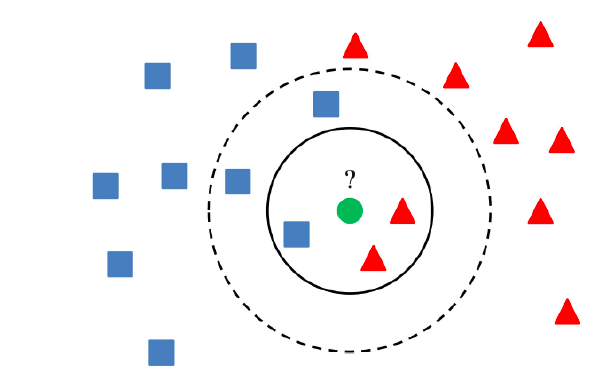
\includegraphics[width=0.8\linewidth]{KNN.png}
	\end{center}
	\caption{Example of a figure embedded in the text.}
	\label{fig:one}
	\end{figure}
	
	\subsection{Simulation Environment}
	The simulations made use of a 80-20 training-testing split, and were run on Google Colab through Python notebooks. Random cross-validation of ten instances was performed, with the final model chosen through averaging of the three most accurate models. Accuracy and area under the curve (AUC) were the main performance measures employed.
	
	\section{Simulation Results}\label{sec:findings}
	\subsection{Key Findings and Significance}
	In this section, the key simulation results and findings are presented concisely. A literature review of related work is also provided, with our results compared against some of this work. It is important to note that our project team only had six weeks to complete the project, and improvements to the methods used could surely have been found had there been more time.
	
	In \cite{einstein}, Thing Two was employed to solve a similar problem, i.e.\ finding the probability of developing sore eyes after 10 hours of gaming, given a set of attributes of the subject consisting mainly of their vital statistics and health condition. In \cite{knuthwebsite}, Thing One and Thing Two were used in a novel combination to solve another biomedical problem, diagnosing the presence of cancer cells in a magnetic resonance imaging (MRI) picture after extracting certain image features. Our novel use of Thing One on its own, with parameters tuned using Method A, proved to be highly competitive against these methods. This is demonstrated in the set of performance curves shown in Figure \ref{fig:two}.
	
	\begin{figure}
	\begin{center}
		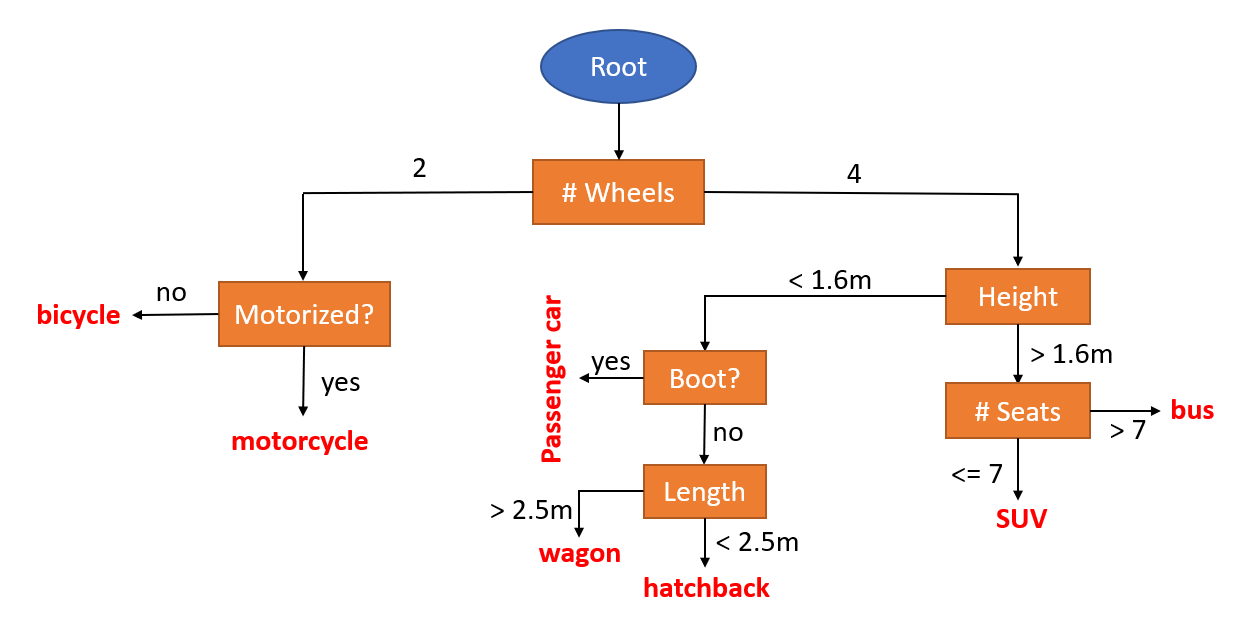
\includegraphics[width=0.8\linewidth]{Dec-Tree.png}
	\end{center}
	\caption{Another example of a figure embedded in the text.}
	\label{fig:two}
	\end{figure}	

	\subsection{Issues Faced} \label{sec:issue}
	The coding of the simulations was not entirely problem-free. We faced the following issues in chronological order, and dealt with them as described.
	\begin{itemize}
		\item Problem One:
		\item Problem Two:
	\end{itemize}

	\section{Potential for Wider Adoption}
	It is encouraging that this short project has produced results that appear to be competitive against the methods proposed by highly regarded research groups. We envisage that future work might include:
	\begin{itemize}
		\item Improvement One
		\item Improvement Two
		\item Adjustment Three
	\end{itemize}

	The interest from industry in this technology is strong, as evidenced by a recent market study conducted by Deloitte \cite{latexcompanion}. Currently, commercial software that is suitable for solving the problem tackled in this project is not available, to our knowledge (after a thorough Internet search). We believe that, after overcoming the issues raised in an earlier section using the methods discussed above, we can build a prototype that can be demonstrated to potential investors. These would include government departments of education, colleges and universities.
	
	\section{Conclusions}
	The project was completed with some degree of success. We managed to do this, that and the other, though not everything in the proposal workplan was completed. The work had to be modified due to the various issues mentioned in Section \ref{sec:issue}. The team worked well together, meeting for at least 2 hours per week, and every team member contributed their fair share of time and effort. The main findings were as follows:
	\begin{enumerate}
		\item Finding One
		\item Finding Two
		\item Finding Three
	\end{enumerate}

	The project can be expanded by capturing more data, and developing more sophisticated methods of classification that could surpass the best result obtained in this project, an accuracy of 85 percent. With an accuracy that approached 95 percent, one could think of commercializing the results either through starting a company or licensing the technology to a company.
		
	%===========================================================
	%===========================================================
	
	\bibliographystyle{ieeetr}
	\bibliography{refs}
	
	
\end{document}